% ---------------------------------------------------------------
% SurjyoPath — The Sun's Way
% Hackathon Presentation
% Compiled with XeLaTeX or pdfLaTeX
% ---------------------------------------------------------------
\documentclass[aspectratio=43, 11pt]{beamer}

%% ---------- Packages ----------
\usepackage[utf8]{inputenc}
\usepackage[T1]{fontenc}
\usepackage{graphicx}
\usepackage{bookmark}
\usepackage{hyperref}
\usepackage{xcolor}
\usepackage{tikz}
\usepackage{microtype}
\usetikzlibrary{shapes.geometric, positioning, arrows.meta, decorations.pathmorphing}

%% ---------- Color Palette (SurjyoPath Galaxy Theme) ----------
\definecolor{SpaceDark}{HTML}{0A0A14}        % deep space
\definecolor{StarGold}{HTML}{F59E0B}         % sun core
\definecolor{SunGlow}{HTML}{F97316}          % orange glow
\definecolor{Corona}{HTML}{FCD34D}           % soft yellow
\definecolor{NebulaPurple}{HTML}{A855F7}     % accent purple
\definecolor{NebulaTeal}{HTML}{14B8A6}       % accent teal
\definecolor{DustGray}{HTML}{9CA3AF}         % muted text
\definecolor{WhiteSoft}{HTML}{F3F4F6}        % soft white

%% ---------- Beamer Theme ----------
\usetheme[numbering=fraction, progressbar=frametitle]{metropolis}
\setbeamercolor{background canvas}{bg=SpaceDark}
\setbeamercolor{normal text}{fg=WhiteSoft}
\setbeamercolor{alerted text}{fg=SunGlow}
\setbeamercolor{example text}{fg=NebulaTeal}
\setbeamercolor{frametitle}{bg=SpaceDark, fg=StarGold}
\setbeamercolor{progress bar}{fg=StarGold, bg=DustGray!30!SpaceDark}
\setbeamercolor{title separator}{fg=StarGold}
\setbeamercolor{structure}{fg=StarGold}
\setbeamercolor{block title}{bg=StarGold!15!SpaceDark, fg=StarGold}
\setbeamercolor{block body}{bg=StarGold!5!SpaceDark, fg=WhiteSoft}
\setbeamercolor{footnote}{fg=DustGray}
\setbeamercolor{page number in head/foot}{fg=DustGray}
\setbeamerfont{footnote}{size=\tiny}

%% ---------- Title Page Decoration ----------
\titlegraphic{
  \begin{tikzpicture}[overlay, remember picture]
    \node[shift={(-3.5cm, -2.5cm)}] at (current page.north east) {
      \begin{tikzpicture}[scale=0.5]
        % Sun glow
        \fill[SunGlow, opacity=0.3] (0,0) circle (4cm);
        \fill[StarGold, opacity=0.5] (0,0) circle (2.5cm);
        \fill[Corona, opacity=0.8] (0,0) circle (1.2cm);
        % Sun icon
        \draw[StarGold, thick, decorate, decoration={snake, amplitude=2mm, segment length=3mm}]
          (0,0) circle (0.8cm);
        % Small orbiting dots
        \foreach \i in {1,...,8} {
          \fill[DustGray] ({2.5*cos(45*\i)}, {2.5*sin(45*\i)}) circle (1.5pt);
        }
      \end{tikzpicture}
    };
  \end{tikzpicture}
}

%% ---------- Meta ----------
\title{\textbf{\textcolor{StarGold}{SurjyoPath}}}
\subtitle{\textit{The Sun's Way} — Your Personal Knowledge Universe}
\author{Team [Your Team Name]}
\date{}

\begin{document}

% ---------------------------------------------------------------
% SLIDE 1 — Title
% ---------------------------------------------------------------
\begin{frame}[plain]
  \vspace{1.5cm}
  \centering
  {\Huge \textbf{\textcolor{StarGold}{SurjyoPath}} \\[0.2cm]}
  {\large \textcolor{Corona}{\textit{The Sun's Way}}}\\[0.4cm]
  {\normalsize \textcolor{DustGray}{A Personal Knowledge Universe}}\\[1cm]

  \begin{center}
    
\begin{tikzpicture}
      \fill[SunGlow, opacity=0.2] (0,0) circle (3.2cm);
      \fill[StarGold, opacity=0.35] (0,0) circle (2cm);
      \fill[Corona, opacity=0.6] (0,0) circle (1cm);
      \fill[StarGold!90!white] (0,0) circle (0.6cm);
      \draw[Corona, thick, decorate, decoration={snake, amplitude=1.5mm, segment length=2.5mm}] (0,0) circle (0.4cm);
    \end{tikzpicture}
  \end{center}

  \vspace{1cm}
  {\small \textcolor{DustGray}{Hackathon Submission --- 2025}}
\end{frame}

% ---------------------------------------------------------------
% SLIDE 2 — Problem
% ---------------------------------------------------------------
\begin{frame}{\textcolor{StarGold}{The Problem}}
  \begin{block}{\textcolor{SunGlow}{Information Overload}}
    Every day we generate thoughts, ideas, goals, and notes --- scattered across apps, notebooks, and memory.
  \end{block}

  \vspace{0.4cm}
  \begin{itemize}
    \item[\textcolor{SunGlow}{$\bullet$}] \textbf{Lost Ideas} --- Great thoughts come and go without capture
    \item[\textcolor{SunGlow}{$\bullet$}] \textbf{No Reflection} --- Journaling feels tedious, not magical
    \item[\textcolor{SunGlow}{$\bullet$}] \textbf{Fragmented Learning} --- Goals, notes, and resources live in silos
    \item[\textcolor{SunGlow}{$\bullet$}] \textbf{Missing Connection} --- No unified space for growth
  \end{itemize}

  \vspace{0.4cm}
  \begin{alertblock}{}
    \centering
    \textit{"I have ideas everywhere, but nowhere to bring them together."}
  \end{alertblock}
\end{frame}

% ---------------------------------------------------------------
% SLIDE 3 — Vision
% ---------------------------------------------------------------
\begin{frame}{\textcolor{StarGold}{The Vision}}
  \centering
  \vspace{0.5cm}
  {\Large \textcolor{Corona}{\textbf{Your ideas orbit around \textit{you}.}}}\\[0.8cm]

  \begin{columns}
    \column{0.45\textwidth}
    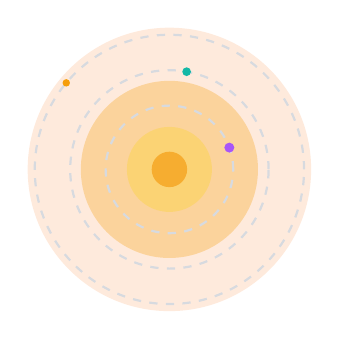
\begin{tikzpicture}[scale=0.45]
      \fill[SunGlow, opacity=0.15] (0,0) circle (4cm);
      \fill[StarGold, opacity=0.3] (0,0) circle (2.5cm);
      \fill[Corona, opacity=0.5] (0,0) circle (1.2cm);
      \fill[StarGold!85!white] (0,0) circle (0.5cm);
      % Orbits
      \draw[DustGray!40, dashed, thick] (0,0) circle (1.8cm);
      \draw[DustGray!40, dashed, thick] (0,0) circle (2.8cm);
      \draw[DustGray!40, dashed, thick] (0,0) circle (3.8cm);
      % Planets
      \fill[NebulaPurple] ({1.8*cos(20)}, {1.8*sin(20)}) circle (4pt);
      \fill[NebulaTeal] ({2.8*cos(80)}, {2.8*sin(80)}) circle (3.5pt);
      \fill[StarGold] ({3.8*cos(140)}, {3.8*sin(140)}) circle (3pt);
    \end{tikzpicture}

    \column{0.55\textwidth}
    \small
    Like a solar system, each of your ideas --- journals, goals, publications, connections --- becomes a celestial body orbiting your personal sun.
    \vspace{0.3cm}

    \textcolor{Corona}{You are the center of your knowledge universe.}
  \end{columns}
\end{frame}

% ---------------------------------------------------------------
% SLIDE 4 — Features
% ---------------------------------------------------------------
\begin{frame}[shrink]{\textcolor{StarGold}{Key Features}}

  \begin{columns}[t]
    \column{0.5\textwidth}
    \begin{block}{\textcolor{SunGlow}{Journal}}
      \small Daily diary with AI-powered thought categorization and reflection prompts
    \end{block}
    \vspace{0.2cm}
    \begin{block}{\textcolor{NebulaPurple}{Goals}}
      \small Set goals with auto-generated learning roadmaps and progress tracking
    \end{block}
    \vspace{0.2cm}
    \begin{block}{\textcolor{NebulaTeal}{Library}}
      \small Save articles, notes, and resources in a personal knowledge base
    \end{block}

    \column{0.5\textwidth}
    \begin{block}{\textcolor{Corona}{Publications}}
      \small Write and publish your thoughts --- turn notes into articles
    \end{block}
    \vspace{0.2cm}
    \begin{block}{\textcolor{StarGold}{Friends}}
      \small Connect with peers, share goals, and grow together
    \end{block}
    \vspace{0.2cm}
    \begin{block}{\textcolor{SunGlow}{Galaxy Navigation}}
      \small A stunning solar-system UI to navigate everything
    \end{block}
  \end{columns}
\end{frame}

% ---------------------------------------------------------------
% SLIDE 5 — Architecture
% ---------------------------------------------------------------
\begin{frame}{\textcolor{StarGold}{How It Works}}

  \centering
  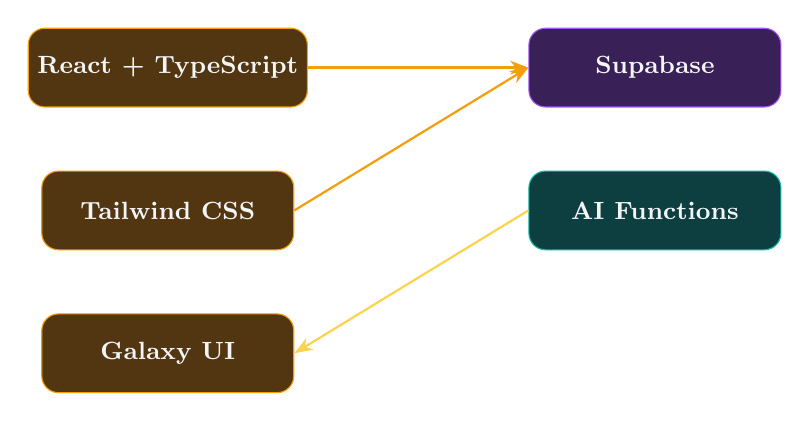
\begin{tikzpicture}[
    node distance=2cm,
    box/.style={
      rectangle, rounded corners=6pt,
      minimum width=3.2cm, minimum height=1cm,
      align=center, font=\small\bfseries,
      text=WhiteSoft
    }
  ]
    %% Frontend
    \node[box, fill=StarGold!30!SpaceDark, draw=StarGold] (react) {React + TypeScript};
    \node[box, fill=StarGold!30!SpaceDark, draw=StarGold, below=0.8cm of react] (ui) {Tailwind CSS};
    \node[box, fill=StarGold!30!SpaceDark, draw=StarGold, below=0.8cm of ui] (nav) {Galaxy UI};

    %% Backend
    \node[box, fill=NebulaPurple!30!SpaceDark, draw=NebulaPurple, right=2.8cm of react] (supa) {Supabase};
    \node[box, fill=NebulaTeal!30!SpaceDark, draw=NebulaTeal, below=0.8cm of supa] (edge) {AI Functions};

    %% Draw arrows
    \draw[StarGold, thick, arrows={-Stealth}] (react.east) -- (supa.west);
    \draw[StarGold, thick, arrows={-Stealth}] (ui.east) -- (supa.west);
    \draw[Corona, thick, arrows={-Stealth}] (edge.west) -- (nav.east);
  \end{tikzpicture}

  \vspace{0.6cm}
  \begin{columns}
    \column{0.33\textwidth}
    \centering
    \textcolor{Corona}{\textbf{Frontend}} \\
    \tiny React, TypeScript, Tailwind v4, Vite

    \column{0.33\textwidth}
    \centering
    \textcolor{NebulaPurple}{\textbf{Backend}} \\
    \tiny Supabase Auth, Postgres, Realtime

    \column{0.33\textwidth}
    \centering
    \textcolor{NebulaTeal}{\textbf{AI}} \\
    \tiny Edge Functions, Thought Analysis, Auto-courses
  \end{columns}
\end{frame}

% ---------------------------------------------------------------
% SLIDE 6 — Tech Stack
% ---------------------------------------------------------------
\begin{frame}{\textcolor{StarGold}{Technology Stack}}

  \centering
  \vspace{0.3cm}
  \begin{tabular}{ll}
    \textcolor{Corona}{\textbf{Frontend}} & React 18, TypeScript, Vite, Tailwind CSS v4 \\
    \textcolor{Corona}{\textbf{State}} & Zustand stores (auth, goals, journal, friends, library, etc.) \\
    \textcolor{NebulaPurple}{\textbf{Backend}} & Supabase (Auth, Postgres, Realtime, Storage) \\
    \textcolor{NebulaPurple}{\textbf{API}} & Supabase Edge Functions (Deno) \\
    \textcolor{NebulaTeal}{\textbf{AI}} & AI-powered thought categorization, learning roadmaps \\
    \textcolor{StarGold}{\textbf{UI/UX}} & Galaxy-themed navigation, dark/light modes, responsive \\
    \textcolor{StarGold}{\textbf{Deploy}} & Vite build, Supabase hosting \\
  \end{tabular}

  \vspace{0.6cm}
  \begin{alertblock}{\textcolor{SunGlow}{Why This Stack?}}
    \small
    Lightning-fast dev with Vite + React, scalable backend with Supabase (no server management), and AI integration via serverless Edge Functions. All TypeScript --- one language from frontend to backend.
  \end{alertblock}
\end{frame}

% ---------------------------------------------------------------
% SLIDE 7 — Design
% ---------------------------------------------------------------
\begin{frame}[shrink]{\textcolor{StarGold}{Design Philosophy}}

  \centering
  \vspace{0.3cm}

  \begin{columns}
    \column{0.45\textwidth}
    \begin{block}{\textcolor{Corona}{Galaxy Metaphor}}
      \small
      Every feature is a planet orbiting your personal sun. Navigation becomes exploration --- intuitive, delightful, memorable.
    \end{block}
    \vspace{0.3cm}
    \begin{block}{\textcolor{NebulaTeal}{Dreamy Animations}}
      \small
      Starburst entrances, pulsing corona glows, slow orbit rotations. Every micro-interaction feels alive.
    \end{block}

    \column{0.45\textwidth}
    \begin{block}{\textcolor{StarGold}{Light \& Dark}}
      \small
      Warm amber-gold sun tones on deep space backgrounds --- with a light mode for daytime use. Accessibility-first.
    \end{block}
    \vspace{0.3cm}
    \begin{block}{\textcolor{DustGray}{Empty States with Soul}}
      \small
      No blank spaces --- every empty state guides the user with personality.
    \end{block}
  \end{columns}
\end{frame}

% ---------------------------------------------------------------
% SLIDE 8 — Impact & Future
% ---------------------------------------------------------------
\begin{frame}{\textcolor{StarGold}{Impact \& Roadmap}}

  \begin{columns}[t]
    \column{0.48\textwidth}
    \textcolor{Corona}{\textbf{Who It Helps}}
    \begin{itemize}
      \item[\textcolor{SunGlow}{--}] Lifelong learners
      \item[\textcolor{SunGlow}{--}] Writers and thinkers
      \item[\textcolor{SunGlow}{--}] Goal-oriented individuals
      \item[\textcolor{SunGlow}{--}] Anyone overwhelmed by information
    \end{itemize}

    \column{0.48\textwidth}
    \textcolor{Corona}{\textbf{Future Roadmap}}
    \begin{itemize}
      \item[\textcolor{NebulaTeal}{$\blacktriangleright$}] Mobile app (React Native)
      \item[\textcolor{NebulaTeal}{$\blacktriangleright$}] Collaborative goal rooms
      \item[\textcolor{NebulaTeal}{$\blacktriangleright$}] AI thought summaries \& insights
      \item[\textcolor{NebulaTeal}{$\blacktriangleright$}] Public publication marketplace
      \item[\textcolor{NebulaTeal}{$\blacktriangleright$}] Offline-first with PWA
    \end{itemize}
  \end{columns}

  \vspace{0.6cm}
  \begin{exampleblock}{\textcolor{NebulaTeal}{Long-term Vision}}
    \centering
    \small
    SurjyoPath aims to be the \textbf{personal operating system for your mind} --- the one place where all your thoughts, goals, and knowledge live, connect, and grow.
  \end{exampleblock}
\end{frame}

% ---------------------------------------------------------------
% SLIDE 9 — Thank You
% ---------------------------------------------------------------
\begin{frame}[plain]
  \vspace{1.5cm}
  \centering

  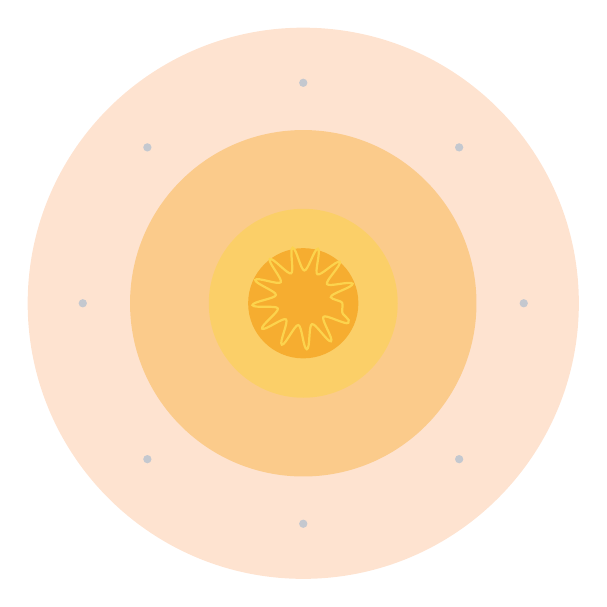
\begin{tikzpicture}
    \fill[SunGlow, opacity=0.2] (0,0) circle (3.5cm);
    \fill[StarGold, opacity=0.35] (0,0) circle (2.2cm);
    \fill[Corona, opacity=0.55] (0,0) circle (1.2cm);
    \fill[StarGold!85!white] (0,0) circle (0.7cm);
    \draw[Corona, thick, decorate, decoration={snake, amplitude=1.5mm, segment length=2.5mm}] (0,0) circle (0.5cm);
    % Tiny orbiting dots
    \foreach \i in {0,45,90,135,180,225,270,315} {
      \fill[DustGray!60] ({2.8*cos(\i)}, {2.8*sin(\i)}) circle (1.5pt);
    }
  \end{tikzpicture}

  \vspace{0.5cm}
  {\Huge \textbf{\textcolor{StarGold}{Thank You}}}\\[0.4cm]
  {\large \textcolor{Corona}{SurjyoPath --- The Sun's Way}}\\[0.2cm]
  {\small \textcolor{DustGray}{May your thoughts shine bright.}}\\[1cm]

  \vfill
  {\tiny \textcolor{DustGray!50}{Built with React, TypeScript, Supabase \& Tailwind CSS}}
\end{frame}

\end{document}